\chapter{用户调研}

\section{技术探针}
为了方便进行用户调研,我们选用了云中医app作为技术探针。云中医是复旦大学计算机学院张文强老师和上海中医药大学合作开发的一款面诊应用,主要为诊所环境使用考虑,虽然没有考虑到用户日常长期使用的情况,但是它实现了面诊,舌诊和问诊的基本功能,符合技术探针的要求。

云中医是一个手机上的健康诊断应用程序,旨在提供一个方便的平台的自我诊断和健康管理。该应用以中医“四诊”理论为指导,用户需要依次对自己的面部和舌头进行拍照,回答一些与自己健康状况相关的问题,最终会收到一份完整的健康报告和一些健康建议。
云中医app的主要界面如\ref{fig:main}所示。

\begin{figure}
    \centering
    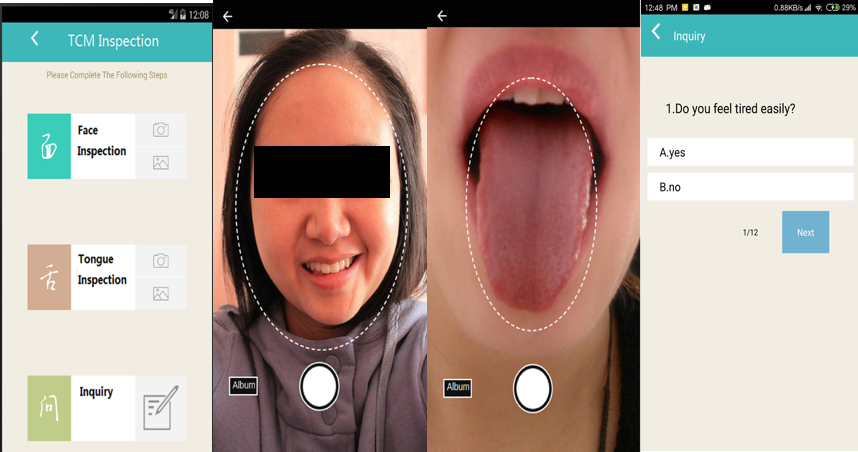
\includegraphics{images/main.png}
    \caption{云中医}
    \label{fig:main}
\end{figure}

\section{调研过程}
 
我们采用定性研究的方法进行半结构化的深度访谈,通过社交媒体发布海报。在被试人员对此应用感兴趣,愿意尝试的前提下,尽量使得招募到的人员在年龄、健康状况、教育背景、工作性质等方面具有多样性。不同的年龄层次可能会导向对健康的不同关注角度(中老年人较为关注的养生知识逐渐在青年群体中流行起来)不同的工作性质使得人们重点关注的身体部位不同(白领普遍关注的肩颈,特殊行业的“职业病”)不同的教育背景使得人们对用技术手段监测健康信息的接受程度也有差异。

通过社交媒体宣传,我们最终招募到了10位感兴趣的志愿者。在招募到合适的用户之后,我们会对每一个用户进行一次采访,主要是为了了解用户信息,介绍技术探针。采访是在征得志愿者的同意下,全程录音的情况下进行的。介绍性的问题大纲如 \ref{tab:inteview_questions}所示。

\begin{table}[]
    
    
    \begin{tabular}{ll}
        \toprule
        编号 & 问题 \\
        \midrule
        1  & 您的年龄?职业背景?   \\
        2  & 您目前健康状况如何?平时感觉身体哪里不舒服吗(慢性病,容易疲劳,关节疼痛等等)?   \\
        3  &  您有使用健康状况评估的技术吗?若有,都有哪些技术?平时如何使用的?使用体验如何?  \\
         4  & 有看多中医吗?是什么原因看的中医?在哪里看的?效果如何?   \\
        5   & 对中医的面诊、舌诊有了解吗?若有,通过什么渠道了解的?   \\
         6  & 平时会留意自己的面色,舌苔吗?会留意其他人的面色,舌苔吗?\\
        7   & 您对这个APP感兴趣的点主要在哪里?\\
        \bottomrule
    \end{tabular}
    \caption{第一次采访问题大纲}
    \label{tab:inteview_questions}
\end{table}

接下来两周时间,在第一星期,我们不做任何干预。而到了第二星期,要求用户每天至少使用一次。在用户使用结束后,我们会进行一次结束后的回访,了解用户在使用中遇到的问题和他们的想法;我们希望通过此次调研了解到使用面诊应用的用户群体有哪些?用户期望通过面诊应用来获取哪方面的信息?以及在方便用户日常使用上,有哪些待解决的技术难点?

\begin{table}
  
  \centering
  \label{tab:Participants}
  \begin{tabular}{llll}
        \toprule
        编号 &	性别 &	年龄 &	职业 \\
        \midrule
        参与者1 &	男 &	20多 &	博士生 \\
        参与者2 &	男 &	20多 &	研究生 \\
        参与者3 &	男 &	20多 &	研究生 \\
        参与者4 &	女 &	50多 &	医院护理工 \\
        参与者5 &	男 &	40多 &	办公室职员 \\
        参与者6 &	女 &	40多 &	小学老师 \\
        参与者7 &	女 &	50多 &	办公室职员 \\
        参与者8 &	女 &	19岁 &	本科生 \\
        参与者9 &	男 &	20多 &	办公室职员 \\
        参与者10 &	女 &	40多 &	办公室职员 \\
        \bottomrule
  \end{tabular}
  \caption{参与者}
\end{table}


\section{调研发现}
通过对采访数据进行分析,我们的用户调研发现如下:
\subsection{潜在的使用场景}
通过调研,我们发现面诊类应用在日常使用环境下,用户反馈有两种潜在的使用场景:

1.了解身体状态

对于那些已经有健康问题的用户或者日常有养生活动的用户对云中医更加感兴趣,并且知道如何在日常生活中使用它。

参与者1他从小就是一个病骨头,总是生病,所以经常看中医。参与者1说道:\textit{“像我这种生了病或者健康状态不好的人,是可以用云中医应用来日常使用来检测疾病的。”}
参与者10对云中医应用也表现出浓厚的兴趣:\textit{“这些诊断结果和建议对我很有用,因为在手机上做诊断很方便,我一有空就会用一用。比如我今天早上有空,我就打开用了一下。”}
参与者3是一个对自己健康状态很看重的人,他说道:\textit{“因为它可以进行面诊和舌诊告诉我结果,并且给出了一定穴位按摩的建议,我觉得很有用。”}

大多数参与者使用云中医不只是为了了解自己身体的状况,更是为了能够及时调整自己的生活方式。
如参与者3有一次早上感觉非常疲倦,于是他拿出云中医应用对自己进行了诊断,果不其然应用给出的分数是自使用以来最低的65分,他觉得这类应用非常重要:\textit{“作为一名学生,久坐是不可避免的。当我感觉疲倦的时候,我就打开云中医看一下,然后根据结果来决定是不是要去锻炼一下。“}
参与者1也提到云中医可以帮助进行健康决策:\textit{“云中医可以帮我了解自己的身体状况,这样我就可以判断自己当天是否可以加班了。“}


2.医患沟通的工具

正如其他健康跟踪类技术的发现类似,参与者希望云中一能够提供医生和患者沟通的渠道,这样医生可以更好地获取病人的日常健康信息。

参与者8说道:\textit{”这类应用可以和医生合作,这样医生就可以获取患者的健康状况并及时发现问题“}, 她进一步建议:\textit{“可以把每次的诊断结果保存到个人档案中,这样医生可以方便地获取到患者的健康信息,这样医生就可以知道患者在就医期间的日常健康状况了。”}

\subsection{自适应性}
日常环境和诊所环境不同,日常环境下需要用户长期使用。但是,大部分的参与者在使用云中医一到两次后就不再使用了,其中一个重要的原因就是云中医缺乏自适应性的能力。

比如参与者1在采访中指出:\textit{”无论我什么时候拍照,它都是问我同样的问题,我会感觉很无聊。“}
同样,参与者2说:\textit{”每次都重复地检查很枯燥。“}参与者6解释了她不继续用云中医的原因:\textit{”一个人的健康状况,在短时间内的变化不会太大,所以我就没一直用了。“}
而参与者7虽然在持续使用,但是也不愿意每次看到相同的信息:\textit{”它每次都给我相同的健康结果,我怀疑它的准确性。”}

参与者在提出问题的同时,也给了对应提高系统自适应性的建议,主要体现在两个方面:

1.自适应用户信息

从调研反馈来看,我们发现因为云中医在问诊的时候,一直问用户同样的问题,而实际情况是短期内来说,大部分问题的答案是不会发生改变的,这样缺乏用户信息的自适应性会让用户使用起来觉得很繁琐。

在这次的用户调研过程中,在诊断应用的场景下,我们发现用户强烈希望系统能够记住他们的用户信息并对下一次诊断进行相应的调整。
比如一些参与者抱怨说每次去回答问诊的问题非常地繁琐, 参与者2说道:\textit{“问诊那一部分设计地不好,每次问题都是固定的,而且太笼统了。”},然后他建议这些问题应该更加个性化:\textit{“我认为问诊的问题可以根据之前问的问题更加地具体。”}
参与者10则希望系统能够追踪用户的健康状况:\textit{“我希望它有后续的追踪过程,不仅可以评估当天的健康状况,也可以在接下来的几天内,跟踪健康问题并动态地调整建议。”}
参与者3也有类似的想法:\textit{“目前系统只有诊断的功能,我希望系统能够接受用户的反馈,比如记录系统给出的健康建议是否有效,这样可以调整健康建议的结果。”}

2.自适应环境信息

系统给出的养生建议也是固定的,并没有考虑到用户当前的工作状态和环境因素。中医认为,于环境变化和谐相处对于保持健康很重要,特别是在季节变化的时候。

参与者6建议:\textit{“养生建议应该更加丰富一些,比如考虑季节和节气的变化。”} 
参与者10希望系统能健康建议和当前天气综合考虑:\textit{“那么热的天气叫我出去运动? 它应该考虑到我个人的健康情况和当前的天气情况。”}

\subsection{实用性}
在调研过程中,我们发现并不是所有的参与者都能接受健康报告的结果,主要原因有以下两个方面:

1.中医术语

云中医应用是和上海中医药大学一起合作研发出来的,健康报告的文字使用的是标准的中医术语。和平时就医环境不同的是,在日常环境下,用户在使用的时候,周围是没有专业的医生可以询问的,因此通俗易懂的解释中医术语是非常重要的。
在调研过程中我们就发现很多参与者很难理解系统给出的健康报告,特别是在年轻群体中,新一代年轻人对中医的接受程度比较低,这个问题就更加严重。
参与者2是在读研究生对健康报告的里“气”的概念就不是很了解,他提到:\textit{“我对中医知之甚少,它说我气虚,但是什么是气虚我都不知道……”}
参与者8也觉得自己对中医知识了解有限,对结果不是很理解:\textit{“分数下面有提到五脏的概念,但是其实我连五脏指的是哪五个器官不是很清楚,可能包括肝脏、心脏和肾脏?”}
虽然中医在中国的历史悠久,但是并不是所有的人都清楚中医中的常见概念。 如果系统是设计给普通用户日常使用的话,就需要考虑到用户的中医知识素养了。

解决此类问题的方法之一,是把中医术语和常见的词语进行关联。比如参与者1遇到这样一个例子:\textit{“我今天感冒了,但是系统却没有提示我感冒了,只是说我气血不畅,它为什么不直接告诉我感冒或者风寒呢?”}

另一个解决方法则是通过更加生动的方式进行介绍,比如视频图片等。还是参与者1,他说:\textit{“健康建议里的按摩,可能直接给出一个按摩的视频,而不是只有文字和图片,有一个视频跟着做的话会更好。”}

参与者还提出可以通过提供学习的机制,让用户了解晦涩的中医术语。
事实上在调研过程中,就有参与者把云中医当作一个学习中医养生的工具,例如参与者10提到:\textit{“我认为系统可以提供更加宽泛的养生知识,而不只是健康建议。我对健康建议中的穴位按摩就很感兴趣。”}

2.养生建议合理性

不同职业的用户,日常的空余时间是不同的。空余时间是否充裕,是影响用户实践养生建议的关键。因此系统给出的养生建议,特别是需要花费较长时间的按摩熬粥之类大的养生活动,需要合理考虑用户的日常空余时间。

比如参与者2就指出:\textit{“作为一个住在没有厨房的公共宿舍的学生,养生建议中的食疗就是不切实际的。我不会做饭,而且有些食物用的材料太贵了,超出了我的承受范围。”}
参与者9是一位刚参加工作的算法工程师,每天8点才下班,他反馈说:\textit{“我基本没有什么时间熬粥或者煎药了。”} 参与者7表示:\textit{“每天都进行穴位按摩太费时间了,我坚持不下来。”}

\subsection{敏感性}
1.文化敏感性

舌诊的时候,需要用户伸出舌头进行拍照。在中国文化中,伸出舌头可以表示厌恶或者无礼,因此在很多情况下,在公众场合伸出自己的舌头被认为是不合适的。如参与者1认为,伸出舌头拍舌头的照片是很不雅的。参与者3表示自己在和别人拍照的时候都会感到紧张,使用云中医时都是私下使用。因此,文化敏感性限制了该类应用的使用范围。

2.技术敏感性

由于模型需要对面部舌部图片进行颜色特征的提取,使其对外部因素如光照和手机摄像头的质量会更加敏感。参与者8还特别反映了自己用的是vivo手机,拍照会受到相机自带美颜算法的影响。因此,将面诊应用日常环境下,需要考虑个人设备的因素。

3.社交敏感性

虽然有几位参与者希望分享它们的健康结果给其他人作为相互学习的机会,但是他们同时也担心因为涉及到面部照片和个人健康信息,可能会导致隐私泄露的问题。


有趣的是,我们发现和其他社交分享类应用不同的是,对于家人来说,他们更加愿意分享给陌生人,因为分享给家人的话可能会引起家人不必要的担心。


\section{}

\section{本章小结}

为了方便后续的实验,本文的主要工作量体现在解决可用性的问题。其中一个重要的工作就是对云中医改造成稳定易用的系统。


可用性(striking a balance, 不需要拍照),透明性  怎么透明性可以提高

为了实现这个实现,我们设计了新的系统

可用性方面,我们做了以下的设计与实现

设计理念,设计方案:

把xxx放到一页,不需要强制顺序
为什么跨平台,提高

再写具体实现,为了方便研究,满足实验的需要。


